% E0240 Project 1, Phase-3 final report (presentations 16-19 November 2026,
% report due 26 November 2026). "WHAT" report from the frozen evidence base
% in PHASE3_EVIDENCE_PACK.md. NOTE: the "Group members" line is the same
% placeholder carried from the earlier reports; fill or delete before
% submission. Every numerical value traces to results/*.csv.
\documentclass[11pt,a4paper]{article}
\usepackage[utf8]{inputenc}
\usepackage[margin=1.5cm,footskip=25pt]{geometry}
\usepackage{amsmath,amssymb}
\usepackage{microtype}
\usepackage{booktabs}
\usepackage{float}
\usepackage{caption}
\captionsetup{font=small,labelfont=bf,skip=4pt}
\usepackage{tikz}
\usetikzlibrary{arrows.meta,positioning,calc}
\usepackage[hidelinks]{hyperref}

\setlength{\parskip}{1.5pt}
\emergencystretch=1em
\makeatletter
\renewcommand\section{\@startsection{section}{1}{\z@}%
  {-3.1ex plus -0.6ex minus -.2ex}{1.6ex plus .2ex}{\normalfont\Large\bfseries}}
\makeatother
\setlength{\intextsep}{4pt plus 1pt minus 1pt}

\title{\vspace{-2.2em}\textbf{\huge E0240: Modeling and Simulation}\\[0.4em]
\Large \textbf{Project Phase-3: Final Report}\\[0.3em]
\large A Queueing-Network Simulator for an LLM Inference Serving Pipeline}
\author{\textbf{Name:} Vaibhav Mahore \quad \textbf{SR No.:} 23631\\[0.2em]
\textit{UG BTech (M\&C)}, Department of Computer Science and Automation (CSA)\\[0.2em]
\textbf{Indian Institute of Science, Bangalore}\\[0.2em]
\textbf{Group members:} \textit{[Name (SR No.)] \quad [Name (SR No.)]}}
\date{\textbf{Submission Date:} 26 November 2026}

\begin{document}
\maketitle
\vspace{-0.4em}
\hrule
\vspace{1.2em}

\section*{1. Introduction and Objective}
In the earlier phases of this project we built a discrete-time queueing-network
simulator for an LLM inference serving pipeline and validated it against the
analytical single-queue models taught in the course; the progress report
described that design and validation. This report answers the question the
simulator was built for: \emph{what does the validated simulator reveal about
the pipeline?} We present three groups of results. First, the validation
evidence that qualifies everything else. Second, a load-response experiment
showing that service variability at the GPU stage is a large delay cost for a
single worker under load, and that a second worker largely removes it.
Third, a batching experiment showing a measurable delay/resource trade-off
with a saturation point in batch size, but no delay-reducing batch
configuration inside the tested grid.

\section*{2. Model and Experimental Setup}
We model the serving pipeline as three stations in a single path (Figure 1):
Q1, admission and tokenization, a Geo/D/1 node with deterministic service
$S_1 = 2$ cycles; Q2, a FCFS batching scheduler that releases a batch when
$B$ requests have collected or the oldest has waited $\tau$ cycles (with
$B=1$, $\tau=0$ a zero-delay pass-through); and Q3, $c$ identical GPU
workers where one worker serves one \emph{batch}: all requests in a batch
share the batch's service duration, with mean $S_3 + \delta(b-1)$ for a
batch of size $b$. Arrivals are Bernoulli with rate $\lambda$ (requests per
cycle; one cycle is one scheduler tick), requests traverse each station once,
and the simulator advances time in fixed increments of one cycle, exactly as
in the course's cycle-driven model. Queue occupancy is the course's
time-average measure, sampled after dispatch and excluding in-service
requests, and all our reported delays are queue waits; every run uses the
fixed seed 20260922. The experiments compare configurations on the same
external arrival stream, so differences between curves reflect the changed
configuration rather than arrival noise.

\begin{figure}[H]
\centering
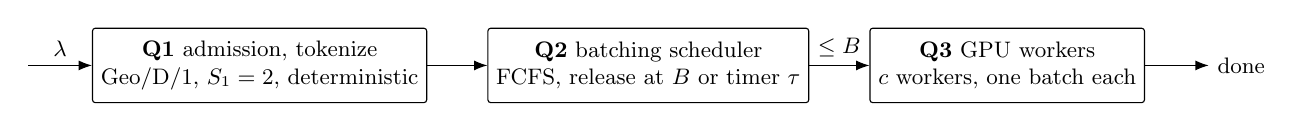
\begin{tikzpicture}[>=Latex, font=\small, scale=0.9, transform shape,
  stn/.style={draw, rounded corners=1pt, minimum width=3.0cm, minimum height=1.05cm, align=center}]
\node[stn] (q1) {\textbf{Q1} admission, tokenize\\ Geo/D/1, $S_1=2$, deterministic};
\node[stn,right=0.85cm of q1] (q2) {\textbf{Q2} batching scheduler\\ FCFS, release at $B$ or timer $\tau$};
\node[stn,right=0.85cm of q2] (q3) {\textbf{Q3} GPU workers\\ $c$ workers, one batch each};
\draw[->] ($(q1.west)+(-0.9,0)$) -- node[above]{$\lambda$} (q1.west);
\draw[->] (q1) -- (q2);
\draw[->] (q2) -- node[above]{$\le B$} (q3);
\draw[->] (q3.east) -- ++(0.9,0) node[right]{done};
\end{tikzpicture}
\caption{The LLM serving pipeline as a three-station queueing network.}
\end{figure}

\section*{3. Validation Summary}
The single-station engine reproduces the discrete-time analytical anchors
(Table 1 summarizes the representative checks).
Against the $S$-general pair $W_q = \rho(S-1)/(2(1-\rho))$ and
$L_q = \lambda W_q$, the worst occupancy error over the stable sweep
($\lambda \le 0.45$, $10^7$ cycles) is 0.75\% at $S=2$ and 0.46\% at $S=3$.
Extending the sweep to $S=3$ showed that the $L_q$ expression we had
initially carried over, $\lambda^2(S-1)/(1-\lambda S)$, is specific to
$S=2$; the $W_q$ expression is the general one and $L_q = \lambda W_q$
follows in our timing convention. With geometric service of mean 2, occupancy
matches $2\lambda^2/(1-2\lambda)$ with worst error 0.94\%, and the simulated
Geo/Geo/1 to Geo/D/1 occupancy ratio stays within 0.95\% of 2 (Figures 2 and
3). At $\lambda = 0.49$ ($\rho = 0.98$) convergence at $10^7$ cycles is slow
(1.1\%), so we treat that point as informational rather than as a pass/fail
row. For the full network we claim no closed form; instead we verify the
simulator's internal accounting: flow balance and network occupancy against
$\lambda W_{\text{e2e}}$ agree to within $3.4\times10^{-7}$, the
$W = L_q/\lambda$ relation per node holds to machine precision, and
utilization and throughput match the offered load within 0.11\%. At the time
of these experiments the course material did not yet include analytical
results for networks, so this consistency evidence is what qualifies the
network model.

\begin{table}[H]
\centering\small
\caption{Representative validation results ($10^7$ cycles; the full table is
in the project package).}
\begin{tabular}{@{}llrrr@{}}
\toprule
Check & Relation & Expected & Simulated & Rel.\ error \\
\midrule
Geo/D/1, $S{=}2$, $\lambda{=}0.45$ & $L_q$ & 2.0250 & 2.0324 & 0.37\% \\
Geo/D/1, $S{=}3$, $\lambda{=}0.30$ & $L_q=\lambda W_q$ & 2.7000 & 2.7118 & 0.44\% \\
Geo/Geo/1, mean 2, $\lambda{=}0.45$ & $L_q$ & 4.0500 & 4.0775 & 0.68\% \\
Occupancy ratio at $\lambda{=}0.45$ & Geo/Geo/1 $:$ Geo/D/1 & 2.0000 & 2.0062 & 0.31\% \\
Pipeline $Q_1$ utilization, $\lambda{=}0.30$ & $\rho_1=\lambda S_1$ & 0.6000 & 0.5997 & 0.06\% \\
\bottomrule
\end{tabular}
\end{table}

\begin{figure}[H]
\centering
\begin{minipage}[t]{0.48\linewidth}
\centering

\includegraphics[width=\linewidth]{figures/fig_e1_validation_geo_d_1.pdf}
\caption{Geo/D/1 validation ($S=2$): occupancy vs injection rate, one curve
per simulation length, against the analytical value. The $10^3$-cycle curve
is off by design; it is the convergence evidence.}
\end{minipage}\hfill
\begin{minipage}[t]{0.48\linewidth}
\centering

\includegraphics[width=\linewidth]{figures/fig_v2_factor2.pdf}
\caption{The factor-2 relationship at $10^7$ cycles: Geo/Geo/1 occupancy is
twice the Geo/D/1 value at equal mean service 2.}
\end{minipage}
\end{figure}

\section*{4. E2: Service Variability and Worker Parallelism}
In this experiment Q2 is a pass-through and Q3 serves one request at a time
(mean service 2), first deterministically and then geometrically, at $c=1$
and $c=2$; compared configurations share the same external arrival stream,
so the curves differ only where the configuration differs.

\textbf{Variability is expensive at high load.} At $\lambda = 0.45$ the mean
end-to-end sojourn rises from 8.519 cycles (deterministic Q3) to 15.350
cycles (geometric Q3, same mean): an increase of 6.831 cycles, or 80.2\%. The
premium is present at every load and grows with it: 2.1\% at $\lambda=0.05$,
23.5\% at $\lambda=0.30$, and 139.9\% at $\lambda=0.49$, where the two
$c=1$ curves reach 28.823 and 69.151 cycles (Figure 4). The mechanism is
visible in the GPU-station occupancy: the geometric curves develop a real
queue (3.08 requests at $\lambda=0.45$) while the deterministic curves do
not (below).

\textbf{A second worker absorbs the penalty.} At $\lambda = 0.45$ the
$c=2$ geometric configuration reaches 8.549 cycles, within 0.03 cycles of
the all-deterministic 8.519; at $\lambda = 0.30$ the same pattern holds
(4.768 against 4.752 at $10^7$ cycles). Under the tested configurations,
parallelism at the GPU stage removes almost the entire delay cost of service
variability.

\textbf{A structural result: the deterministic tandem never builds a GPU
queue.} In all 22 deterministic-configuration rows (both $c$ values, all ten
loads, at $10^6$ and $10^7$ cycles) the Q3 occupancy is exactly zero. This
is not a coincidence but a property of the tested configuration
($S_1 = S_3 = 2$ deterministic, pass-through Q2): a single deterministic
server with $S_1 = 2$ cannot produce two completions closer than 2 cycles
apart, so Q3's arrivals are spaced at least 2 cycles; a 2-cycle service that
starts at cycle $t$ frees its worker during cycle $t+2$'s service step,
which precedes that cycle's dispatch, so even the earliest possible arrival
starts immediately and the queue can never grow. Additional workers only
add capacity. We state this as a result for this configuration, not as a
property of queueing networks in general.

\begin{figure}[H]
\centering

\includegraphics[width=0.8\linewidth]{figures/fig_e2_e2e_delay.pdf}
\caption{E2: end-to-end delay vs injection rate (B = 1, $10^6$-cycle sweep,
paired arrival streams). Geometric service at $c=1$ dominates; $c=2$
essentially removes the penalty.}
\end{figure}

\section*{5. E3: The Batching Trade-off}
Here Q2 batches (release at $B$ collected or timer $\tau$) and Q3's batch
service is $\lceil 2 + 0.5(b-1)\rceil$ cycles for a batch of size $b$
($\delta = 0.5$), at $\lambda = 0.3$. Table 2 shows the $10^7$-cycle grid;
runs at $10^6$ cycles agree with it to at most 0.004 cycles on sojourn
(maximum relative difference 0.29\% across the grid's five metrics), so the
conclusions below are length-robust.

\begin{table}[H]
\centering\small
\caption{E3 results at $\lambda = 0.3$, $\delta = 0.5$, $10^7$ cycles.}
\begin{tabular}{@{}rrrrrrr@{}}
\toprule
$B$ & $\tau$ & Mean fill & Sojourn (cyc) & $Q_2$ wait (cyc) & $Q_3$ util. & Throughput \\
\midrule
1 & 2 & 1.00 & 4.752 & 0.752 & 0.5999 & 0.3000 \\
1 & 8 & 1.00 & 4.752 & 0.752 & 0.5999 & 0.3000 \\
2 & 2 & 1.57 & 6.752 & 2.023 & 0.4906 & 0.3000 \\
2 & 8 & 1.95 & 7.360 & 2.384 & 0.4536 & 0.3000 \\
4 & 8 & 3.17 & 10.438 & 4.875 & 0.3224 & 0.3000 \\
8 & 2 & 1.57 & 6.752 & 2.023 & 0.4906 & 0.3000 \\
8 & 8 & 3.33 & 10.969 & 5.391 & 0.3063 & 0.3000 \\
16 & 8 & 3.33 & 10.969 & 5.391 & 0.3063 & 0.3000 \\
\bottomrule
\end{tabular}
\end{table}

We observe four things. (i) \emph{Batching trades waiting for efficiency.}
Larger batches cut the per-worker utilization nearly in half (0.5999 at
$B=1$ to 0.3063 at $B=8$, $\tau=8$) because the batch service grows
sublinearly (2.000 to 3.400 cycles per batch of mean fill 3.33), but the
saved service time is outweighed by the added $Q_2$ waiting: in this grid
the lowest end-to-end delay occurs at $B=1$, and delay rises with batching
at both timer settings. (ii) \emph{At $\tau=2$, batch size is inert.} The
timer releases requests long before $B$ accumulate, so the rows for
$B = 2, 4, 8, 16$ are identical in every recorded metric (mean fill 1.57).
(iii) \emph{At $\tau=8$ the response saturates between $B=4$ and $B=8$}:
fill grows 1.95, 3.17, 3.33 and then stops, and the $B=8$ and $B=16$ rows
are identical in every recorded metric; we call this an empirical saturation
knee, not an optimum. (iv) \emph{Throughput does not respond} to batching in
the tested stable regime: it stays within 0.06\% of $\lambda = 0.3$ in all
twenty runs, so batching changes delay and resource utilization, not
delivered rate (Figure 5).

\begin{figure}[H]
\centering

\includegraphics[width=0.95\linewidth]{figures/fig_e3_batching.pdf}
\caption{E3: end-to-end sojourn, throughput, and mean batch fill vs batch
size ($\lambda = 0.3$, $\delta = 0.5$, $10^7$ cycles, paired arrival
streams). The fill and delay curves saturate between $B=4$ and $B=8$ at
$\tau=8$.}
\end{figure}

\section*{6. Limitations}
Our conclusions hold inside the tested model, and six of its boundaries
matter most. The network is a linear feedforward chain with a single
Bernoulli external input, so splits, feedback, and burstier arrivals are
outside the evidence. Batching is static (a batch is closed at release) and
the batching gain is a configured sublinear law, not a measured GPU cost
model. Service is restricted to deterministic and geometric laws, and time
is tick-quantized with whole-cycle delays. Queues are unbounded: there is no
admission control, so saturation appears as growing delay rather than
rejected requests. Network-level analytical validation is not part of our
evidence base yet, since the corresponding course material had not been
covered at experiment time. Finally, the cycle-to-scheduler-tick mapping is
representative rather than calibrated against a measured serving system.

\section*{7. Conclusion}
Three messages survive the whole study. First, our simulator is strongly
validated: its single-station behavior matches the course's discrete-time
analytical results to within 1\% at every converged load, including the
factor-2 relationship between deterministic and geometric service, and the
network passes every internal flow and accounting check. Second, service
variability and worker parallelism materially shape latency under load: at
$\lambda = 0.45$, geometric decode service costs 80.2\% extra end-to-end
delay at one worker in the paired-arrival experiment, and a second worker
removes almost all of it, while a deterministic tandem with matched service
times sustains an empty GPU queue as a structural property of its timing.
Third, batching exhibits a measurable delay/resource trade-off with an
empirical saturation point between batch sizes 4 and 8 at the longer timer,
but no batch configuration in the tested grid reduces delay below no
batching at $\lambda = 0.3$; within the stable regime, batching changes
delay and utilization rather than throughput. The simulator and its evidence
base are one-command reproducible, and extending the validation with
analytical network results remains open as the corresponding course material
becomes available.

\end{document}
